\section{Introduction}
\label{sec:introduction}

\begin{frame}{Sample frame title}
  This is a text in the first frame. This is a text in first frame. This is a
  text in first frame. DUMMY
\end{frame}

\begin{frame}{State of the Art}

  \begin{enumerate}
    \item Estimeate reactor temperatures for an assumed power distribution.
    \item Calculate thermally expanded dimensions for reactor assemblies.
    \item Calculate number densities and area fractions to homogenize
      assemblies.
    \item Use assembly-homogenized number densities to calculate material
      cross-sections in zero-dimension transport solution in \mcc.
    \item Model homogenized-assembly compositions in \dif and run.
    \item Collect \keff and multigroup scalar fluxes.
  \end{enumerate}

  \begin{block}{}
    No capabilities for thermal hydraulic analysis or thermal expansion
    analysis.
  \end{block}
\end{frame}

\begin{frame}{Proposed Method}
  \begin{enumerate}
    \item Use similar procedure to generate cross-sections using \mcc.
    \item User inputs pin data that is internally homogenized.
    \item Simulate thermal expansion and thermal hydraulics internally.
    \item Collect \keff, multigroup scalar fluxes, reactor power, and average
      reactor temperatures.
  \end{enumerate}
  %\\
  \begin{itemize}
    \item Thermal expansion and thermal hydraulic simulations have been moved
      internally and are now inherent to the simulation.
    \item Thermal hydraulic simulation also improves the accuracy of neutronics
      simulation by leading to more accurate cross sections.
  \end{itemize}
\end{frame}

\begin{frame}
  \begin{figure}
    \centering
    \includegraphics[width=0.9\textwidth]{reactor_materials}
    \caption{Example of Fast Reactor Materials based on MONJU.}
    \label{fig:reactor_materials}
  \end{figure}
\end{frame}

\begin{frame}
  \begin{figure}
    \centering
    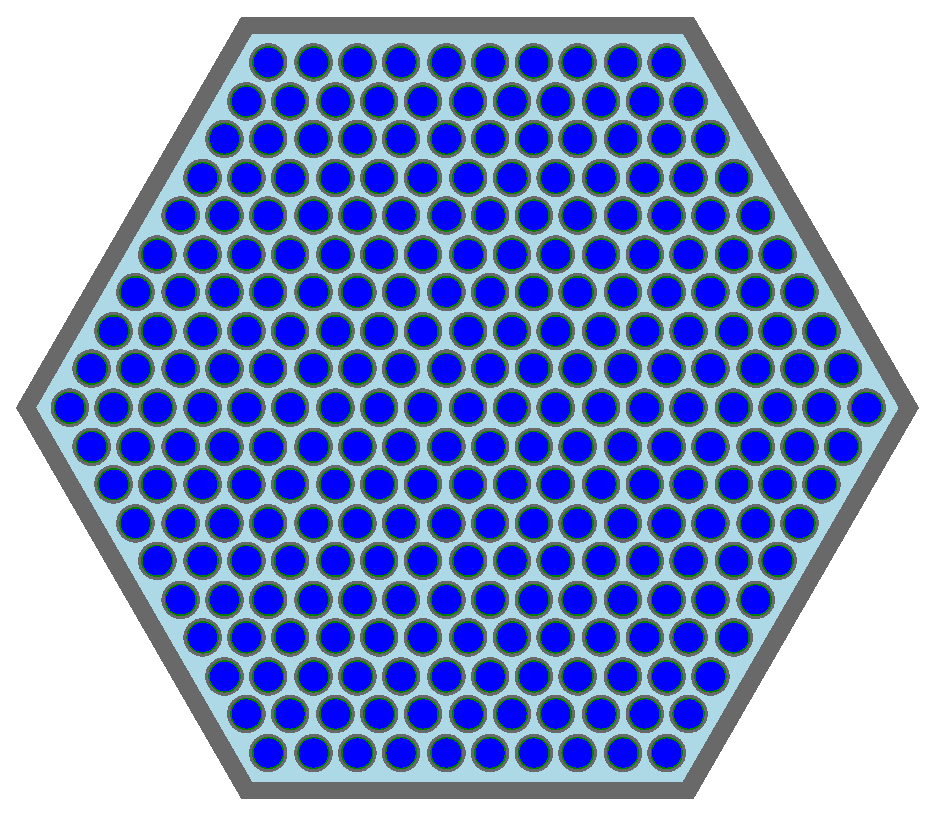
\includegraphics[width=0.5\textwidth]{prism_hex}
    \caption{Example of Fast Reactor Fuel Assembly Cross-Section.}
    \label{fig:prism_hex}
  \end{figure}
\end{frame}

\begin{frame}
  \begin{figure}
    \centering
    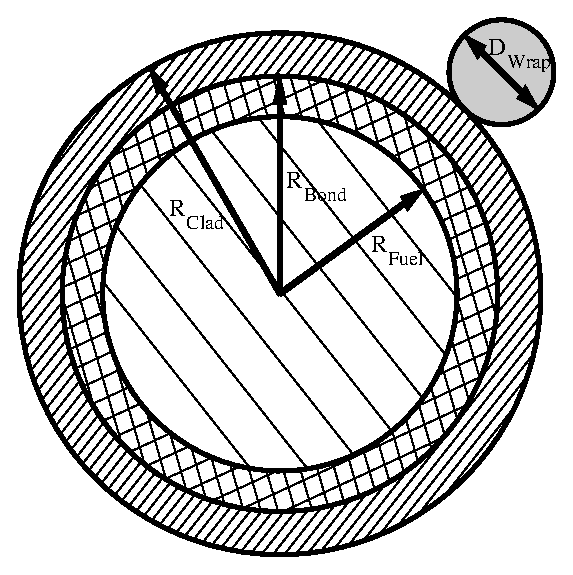
\includegraphics[width=0.5\textwidth]{pin_model}
    \caption{Dimensions of Thermal Hydraulic Rod Model.}
    \label{fig:pin_model}
  \end{figure}
\end{frame}

\begin{frame}
  \begin{figure}
    \centering
    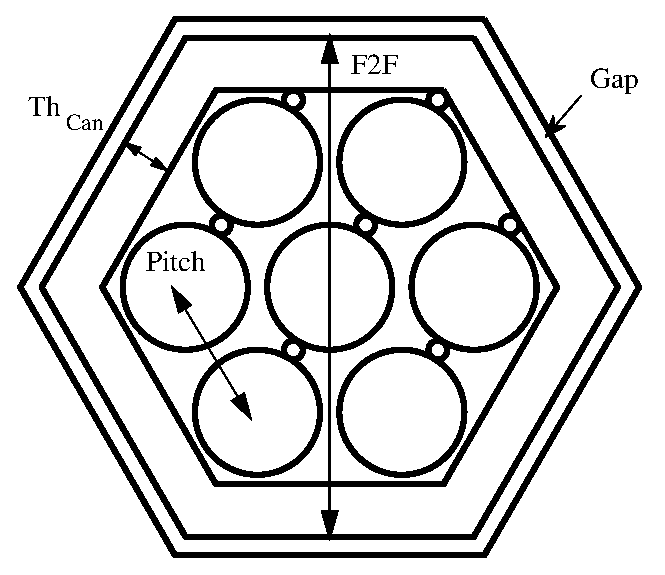
\includegraphics[width=0.5\textwidth]{hex_can}
    \caption{Dimensions of Hexagonal Can.}
    \label{fig:hex_can}
  \end{figure}
\end{frame}

